%!TEX root = slide.tex

\section{Subprogramas como parâmetro}
\begin{frame}{Subprogramas como parâmetro}
	\begin{itemize}
	  \item Ideia simples, mas gera complicações.
	  \item \emph{Type checking}.
	  \item referencing environment.
	\end{itemize}
\end{frame}

\begin{frame}{Referencing Environment}
	\begin{itemize}
	  \item Linguagens que permitem subprogramas aninhados.
	  \item Shallow Binding
	  \item Deep Binding
	  \item Ad Hoc Binding
	\end{itemize}
\end{frame}

\begin{frame}{Exemplo}
	\begin{figure}[ht!]
		\centering
		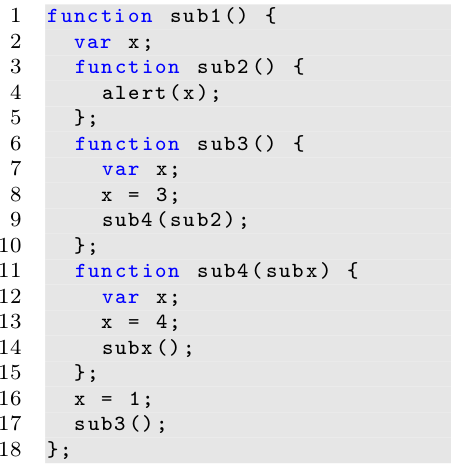
\includegraphics[scale=0.4]{./imgs/js-original}
	\end{figure}
\end{frame}

\begin{frame}{Shallow Binding}
	O ambiente é o local onde o subprograma é chamado.
\end{frame}

\begin{frame}{Shallow Binding}
	\begin{figure}[ht!]
		\centering
		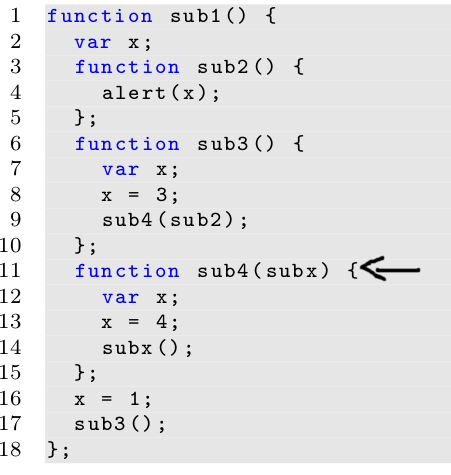
\includegraphics[scale=0.4]{./imgs/js-shallow}
	\end{figure}
\end{frame}

\begin{frame}{Deep Binding}
	O ambiente refere-se onde o subprograma foi definido.
\end{frame}

\begin{frame}{Deep Binding}
	\begin{figure}[ht!]
		\centering
		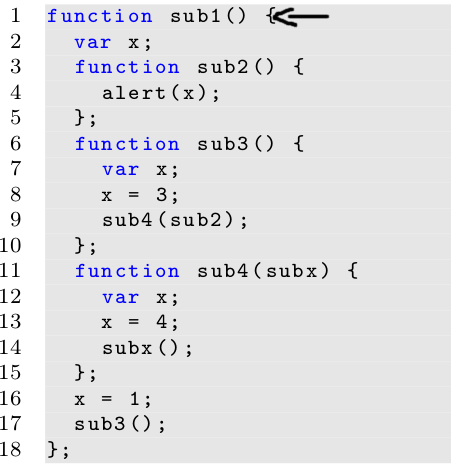
\includegraphics[scale=0.4]{./imgs/js-deep}
	\end{figure}
\end{frame}

\begin{frame}{Ad Hoc Binding}
	O ambiente condiz com o local que o subprograma foi passado por parâmetro.
	Nunca implementado.
\end{frame}

\begin{frame}{Ad Hoc Binding}
	\begin{figure}[ht!]
		\centering
		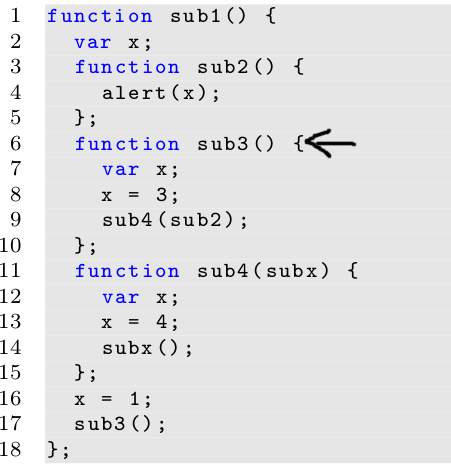
\includegraphics[scale=0.4]{./imgs/js-adhoc}
	\end{figure}
\end{frame}
